
\documentclass[aspectratio=169]{beamer}
\usepackage{animate}
\usepackage{tikz}
\usepackage{svg}
\usepackage{graphicx}
\usetheme{metropolis}

% Define the footer globally in the theme configuration
\setbeamertemplate{footline}{
    \leavevmode%
    \hbox{%
        \begin{beamercolorbox}[wd=.33\paperwidth,ht=2.5ex,dp=1ex,leftskip=3mm]{author in head/foot}%
            \tiny Sam Leeney
        \end{beamercolorbox}%
        \begin{beamercolorbox}[wd=.33\paperwidth,ht=2.5ex,dp=1ex,center]{title in head/foot}%
            \tiny sakl2@cam.ac.uk
        \end{beamercolorbox}%
        \begin{beamercolorbox}[wd=.33\paperwidth,ht=2.5ex,dp=1ex,rightskip=3mm]{date in head/foot}%
            \tiny \href{https://github.com/samleeney}{github.com/samleeney/Talks}
        \end{beamercolorbox}%
    }%
    \vskip0pt%
}

\begin{document}

\begin{frame}
	\begin{center}
		% Title
		{\LARGE Calibration with Machine Learning for REACH\par}
		\vspace{0.5cm}

		% First Author
		{\large Samuel Alan Kossoff Leeney\par}
		\vspace{0.5cm}

		% Institute
		{\normalsize Reach Annual Meeting 2024\par}

		% Date
		{\normalsize 26 September \par}
		\vspace{1cm}

		% Co-authors
		{\footnotesize Co Authors: Harry Bevins, Will Handley, Eloy de Lera Acedo, Christian Kirkhan, Jiacong Zhu, Kaan Artuc, Daniel Molnar\par}
		\vfill

		% Image at the bottom
		
\includegraphics[width=0.9\textwidth]{affiliations.png}
	\end{center}
\end{frame}

\begin{frame}{\small{What is calibration?}}
	\begin{figure}[h]
		\centering
		\includesvg[width=0.6\textwidth]{whatiscal.svg}
	\end{figure}
	\vfill
\end{frame}

\begin{frame}{\small{How to calibrate?}}
	\begin{figure}[h]
		\centering
		\includesvg[width=0.65\textwidth]{howtocal.svg}
	\end{figure}
	\vspace{0.7cm}
	\vfill
\end{frame}

\begin{frame}{\small{Why is calibration in Global 21cm Cosmology difficult?}}
	\begin{figure}[h]
		\centering
		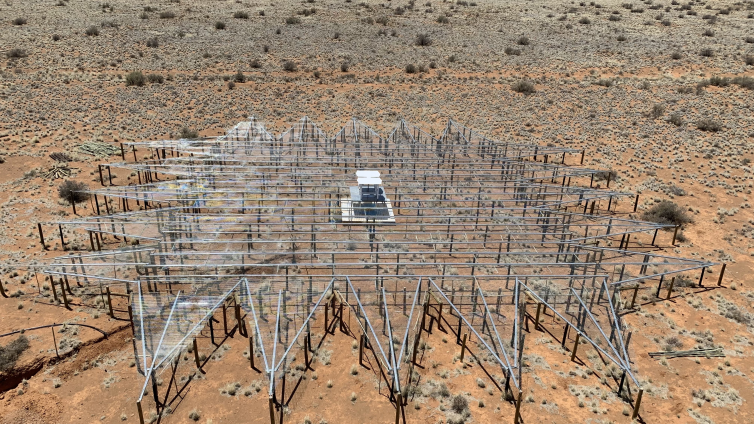
\includegraphics[width=0.6\textwidth]{antenna.png}
	\end{figure}

	\begin{center}
		\begin{tikzpicture}
			\node[draw, rounded corners, inner sep=10pt] (box) {%
				\begin{minipage}{0.9\textwidth} % Width of the box
					\begin{columns}[c] % Align columns centrally inside the box
						\begin{column}{0.33\textwidth}
							\centering
							{\small We measure \textit{sky averaged} signal.}
						\end{column}
						\begin{column}{0.33\textwidth}
							\centering
							{\small Antenna  LNA impedance mismatch}
						\end{column}
						\begin{column}{0.33\textwidth}
							\centering
							{\small Very faint signal.}
						\end{column}
					\end{columns}
				\end{minipage}
			};
		\end{tikzpicture}
	\end{center}

\end{frame}

\begin{frame}{\small{How to calibrate (in a bit more detail...)?}}
	\vspace{-0.5cm}
	\begin{flushleft}
		\textbf{Objective:} Map input temperature to output power.
		\vspace{0.2cm}

		\textbf{Key Factors:}
		\begin{itemize}
			\item LNA introduces time-dependent gain, $g(t)$.
			\item Impedance mismatch adds noise ($T_{\text{rec}}$) to the system.
		\end{itemize}

		\vspace{0.2cm}
		\textbf{Link Output Power to Input Temperature:}
	\end{flushleft}

	% Apply \tiny to the entire equation by wrapping it in a group
	{
	\begin{equation}
		P_{\text{out}}^{\text{src}} = g M \left( T_{\text{in}}^{\text{src}} + T_{\text{rec}} \right)
	\end{equation}
	}

	\vfill % Pushes the following content to the bottom

	\begin{footnotesize}
		\textit{Note: All parameters above are frequency-dependent, but the notation has been simplified here and thereafter for convenience.}
	\end{footnotesize}

\end{frame}

\begin{frame}{\small{Dealing with reflections...}}

	% Output Power Equation without title, maintaining the same equation number (1)
	{\tiny
		\begin{equation}
			P_{\text{out}}^{\text{src}} = \textcolor{red}{g} M \left( T_{\text{in}}^{\text{src}} + \textcolor{red}{T_{\text{rec}}} \right)
		\end{equation}
	}

	\vspace{0.3cm}
	\hrule  % Horizontal line for separation
	\vspace{0.3cm}

	% Noise Parameter Equation with smaller, uniform title
	\textbf{\small{Noise Parameter Equation:}}
	{\tiny
		\begin{equation}
			P_{\text{out}}^{\text{src}} = \textcolor{red}{g} M \left( T_{\text{in}}^{\text{src}} + \textcolor{red}{T_{\text{min}}} + T_0 \frac{4\textcolor{red}{R_N}}{Z_0} \frac{|\Gamma_{\text{src}} - \textcolor{red}{\Gamma_{\text{opt}}}|^2}{(1 - |\Gamma_{\text{src}}|^2)(1 + |\Gamma_{\text{opt}}|^2)} \right)
		\end{equation}
	}

	\vspace{0.3cm}
	\hrule  % Horizontal line for separation
	\vspace{0.3cm}

	% Noise Wave Equation with smaller, uniform title
	\textbf{\small{Noise Wave Equation:}}

	{\tiny
		\begin{multline}\label{}
			P_{\text{out}}^{\text{src}} = \textcolor{red}{g} \left[ \textcolor{red}{T_0} + \textcolor{red}{T_{\text{unc}}} |\Gamma_{\text{s}}|^2 \left|\frac{ \sqrt{1 - |\Gamma_{\text{rec}}|^2}}{1 - \Gamma_{\text{s}}\Gamma_{\text{rec}}} \right|^2 \right. \\
				\left. + T_{\text{s}}(1 - |\Gamma_{\text{s}}|^2) \left|\frac{ \sqrt{1 - |\Gamma_{\text{rec}}|^2}}{1 - \Gamma_{\text{s}}\Gamma_{\text{rec}}} \right|^2 + \textcolor{red}{T_{\text{cos}}} \Re \left( \Gamma_{\text{s}} \frac{\sqrt{1 - |\Gamma_{\text{rec}}|^2}}{1 - \Gamma_{\text{s}} \Gamma_{\text{rec}}} \right) \right. \\
				\left. + \textcolor{red}{T_{\text{sin}}} \Im \left( \Gamma_{\text{s}} \frac{\sqrt{1 - |\Gamma_{\text{rec}}|^2}}{1 - \Gamma_{\text{s}} \Gamma_{\text{rec}}} \right) \right]
		\end{multline}
	}

\end{frame}

\begin{frame}{\small{Calibration Equation}}

	\vspace{0.2cm} % Adds a small vertical space at the top

	\textbf{Typically, substitute in the noise wave parameter equation here (gains cancel)}

	\vspace{0.2cm} % Adds space between text and first equation

	% Calibration Equation with \tiny font and manual tag (4)
	{\tiny
		\begin{equation}
			T_{\text{cal}}^* = T_{\text{NS}} \frac{P_{\text{cal}} - P_L}{P_{\text{NS}} - P_L} + T_L \tag{4}
		\end{equation}
	}

	\vspace{0.3cm} % Adds space between equation and next text

	\textbf{Make some matching assumptions and re arrange:}

	\vspace{0.2cm} % Adds space between text and second equation

	% Multline Equation with \tiny font and manual tag (5)
	{\tiny
		\begin{multline}
			T_\mathrm{s} = \textcolor{red}{T_\mathrm{NS}}\left(\frac{P_\mathrm{s} - P_\mathrm{L}}{P_\mathrm{NS} - P_\mathrm{L}}\right)\frac{\left|1 - \Gamma_\mathrm{s}\Gamma_\mathrm{rec}\right|^2}{1 - |\Gamma_\mathrm{s}|^2} + \textcolor{red}{T_\mathrm{L}}\frac{\left|1 - \Gamma_\mathrm{s}\Gamma_\mathrm{rec}\right|^2}{1 - |\Gamma_\mathrm{s}|^2} - \textcolor{red}{T_\mathrm{unc}} \frac{|\Gamma_\mathrm{s}|^2}{1 - |\Gamma_\mathrm{s}|^2} +  \\
			-\textcolor{red}{T_\mathrm{cos}} \frac{\Re \left( \frac{\Gamma_\mathrm{s}}{1 - \Gamma_\mathrm{s}\Gamma_\mathrm{rec}} \right)\left|1 - \Gamma_\mathrm{s}\Gamma_\mathrm{rec}\right|^2}{(1 - |\Gamma_\mathrm{s}|^2) \sqrt{1 - |\Gamma_\mathrm{rec}|^2}}  -\textcolor{red}{T_\mathrm{sin}} \frac{\Im \left( \frac{\Gamma_\mathrm{s}}{1 - \Gamma_\mathrm{s}\Gamma_\mathrm{rec}} \right)\left|1 - \Gamma_\mathrm{s}\Gamma_\mathrm{rec}\right|^2}{(1 - |\Gamma_\mathrm{s}|^2) \sqrt{1 - |\Gamma_\mathrm{rec}|^2}} \tag{5}
		\end{multline}
	}

	\textit{Note: We end up with 5 parameters that need to be estimated to calibrate the system.}

	\vfill % Pushes the note to the bottom
\end{frame}

\begin{frame}{Calculating the error}

	% Adding a block
	\textbf{By partial derivatives}
	To find the error in \( T_s \), we propagate the errors in \( \Gamma_s \), \( \Gamma_{rec} \), \( P_L \), \( P_{NS} \), and \( P_s \):
	%
	\begin{multline}
		(\Delta T_s)^2 = \left(\frac{\partial T_s}{\partial \Gamma_s} \Delta \Gamma_s\right)^2 + \left(\frac{\partial T_s}{\partial \Gamma_{rec}} \Delta \Gamma_{rec}\right)^2 \\ + \left(\frac{\partial T_s}{\partial P_L} \Delta P_L\right)^2 + \left(\frac{\partial T_s}{\partial P_{NS}} \Delta P_{NS}\right)^2 + \left(\frac{\partial T_s}{\partial P_s} \Delta P_s\right)^2.
	\end{multline}
	%

\end{frame}

\begin{frame}{Calculating the error}
	\vfill
	{\tiny
		\begin{multline}
			(\Delta T_s)^2 =
			\left(\frac{\partial T_s}{\partial \Gamma_s} \Delta \Gamma_s\right)^2 +
			\left(\frac{\partial T_s}{\partial \Gamma_{rec}} \Delta \Gamma_{rec}\right)^2 +
			\left(\frac{\partial T_s}{\partial P_L} \Delta P_L\right)^2 +
			\left(\frac{\partial T_s}{\partial P_{NS}} \Delta P_{NS}\right)^2 +
			\left(\frac{\partial T_s}{\partial P_s} \Delta P_s\right)^2.
		\end{multline}
	}

	\hrule

	\begin{columns}[c] % Align columns centrally inside the box
		\begin{column}{0.4\textwidth}
			\centering
			{\tiny
				\begin{align}
					\frac{\partial T_s}{\partial P_L}    & = T_\mathrm{NS} \frac{\left|1 - \Gamma_\mathrm{s} \Gamma_\mathrm{rec}\right|^2}{1 - |\Gamma_\mathrm{s}|^2} \cdot \frac{P_\mathrm{s} - P_\mathrm{NS}}{(P_\mathrm{NS} - P_\mathrm{L})^2}, \\
					\frac{\partial T_s}{\partial P_{NS}} & = -T_\mathrm{NS} \frac{\left|1 - \Gamma_\mathrm{s} \Gamma_\mathrm{rec}\right|^2}{1 - |\Gamma_\mathrm{s}|^2} \cdot \frac{P_\mathrm{s} - P_\mathrm{L}}{(P_\mathrm{NS} - P_\mathrm{L})^2}, \\
					\frac{\partial T_s}{\partial P_s}    & = T_\mathrm{NS} \left(\frac{1}{P_\mathrm{NS}-P_\mathrm{L}}\right) \frac{\left|1-\Gamma_\mathrm{s}\Gamma_\mathrm{rec}\right|^2}{ 1-|\Gamma_\mathrm{s}|^2}.
				\end{align}

				\begin{equation}
					\frac{\partial T_s}{\partial \Gamma_{rec}} = \frac{\partial A}{\partial \Gamma_{rec}} + \frac{\partial B}{\partial \Gamma_{rec}} + \frac{\partial D}{\partial \Gamma_{rec}} + \frac{\partial E}{\partial \Gamma_{rec}}.
				\end{equation}

				\begin{equation}
					\frac{\partial T_s}{\partial \Gamma_s} = \frac{\partial A}{\partial \Gamma_s} + \frac{\partial B}{\partial \Gamma_s} + \frac{\partial C}{\partial \Gamma_s} + \frac{\partial D}{\partial \Gamma_s} + \frac{\partial E}{\partial \Gamma_s}.
				\end{equation}
			}
		\end{column}

		\begin{column}{0.6\textwidth}
			{\tiny
				\begin{align}
					A & = T_\mathrm{NS}\left(\frac{P_\mathrm{s} - P_\mathrm{L}}{P_\mathrm{NS}-P_\mathrm{L}}\right)\frac{\left|1-\Gamma_\mathrm{s}\Gamma_\mathrm{rec}\right|^2}{ 1-|\Gamma_\mathrm{s}|^2},                                               \\
					B & = T_\mathrm{L}\frac{\left|1-\Gamma_\mathrm{s}\Gamma_\mathrm{rec}\right|^2}{ 1-|\Gamma_\mathrm{s}|^2},                                                                                                                           \\
					C & = - T_\mathrm{unc} \frac{ |\Gamma_\mathrm{s}|^2}{1-\left|\Gamma_\mathrm{s}\right|^2},                                                                                                                                           \\
					D & = -T_\mathrm{cos} \frac{\Re \left( \frac{ \Gamma_\mathrm{s}}{1-\Gamma_\mathrm{s}\Gamma_\mathrm{rec}}\right)\left|1-\Gamma_\mathrm{s}\Gamma_\mathrm{rec}\right|^2}{( 1-|\Gamma_\mathrm{s}|^2) \sqrt{1-|\Gamma_\mathrm{rec}|^2}}, \\
					E & = -T_\mathrm{sin} \frac{\Im \left( \frac{ \Gamma_\mathrm{s}}{1-\Gamma_\mathrm{s}\Gamma_\mathrm{rec}}\right)\left|1-\Gamma_\mathrm{s}\Gamma_\mathrm{rec}\right|^2}{( 1-|\Gamma_\mathrm{s}|^2) \sqrt{1-|\Gamma_\mathrm{rec}|^2}}.
				\end{align}
			}
		\end{column}
	\end{columns}
\end{frame}

\begin{frame}{Calculating the error}

	% Adding a block
	\textbf{Using $T_{\text{NS}} \frac{P_{\text{cal}} - P_L}{P_{\text{NS}} - P_L} + T_L$}
	%
	\begin{align}
		(\Delta T_s)^2 & = \left(\frac{\partial T_s}{\partial P_s} \Delta P_s\right)^2 + \left(\frac{\partial T_s}{\partial P_L} \Delta P_L\right)^2 + \left(\frac{\partial T_s}{\partial P_{NS}} \Delta P_{NS}\right)^2 \\ &+ \left(\frac{\partial T_s}{\partial \Gamma_s} \Delta \Gamma_s\right)^2 + \left(\frac{\partial T_s}{\partial \Gamma_{rec}} \Delta \Gamma_{rec}\right)^2.
	\end{align}
	%

	\hrule
	\textbf{Using noise wave parameters \textit{only}}
	%
	\begin{align}
		(\Delta T_\mathrm{s})^2 & = \left(\frac{\partial T_\mathrm{s}}{\partial P_\mathrm{s}} \Delta P_\mathrm{s}\right)^2 \\ &+ \left(\frac{\partial T_\mathrm{s}}{\partial \Gamma_\mathrm{s}} \Delta \Gamma_\mathrm{s}\right)^2 + \left(\frac{\partial T_\mathrm{s}}{\partial \Gamma_\mathrm{rec}} \Delta \Gamma_\mathrm{rec}\right)^2.
	\end{align}
	%
	\textit{Note that this argument applies for both noise parameters and noise wave parameters.}

\end{frame}

\begin{frame}

	\begin{columns}
		\begin{column}{0.2\textwidth}
			There is more noise when using $T_{\text{NS}} \frac{P_{\text{cal}} - P_L}{P_{\text{NS}} - P_L} + T_L$
		\end{column}
		\begin{column}{0.8\textwidth}
			\begin{figure}[h]
				\centering
				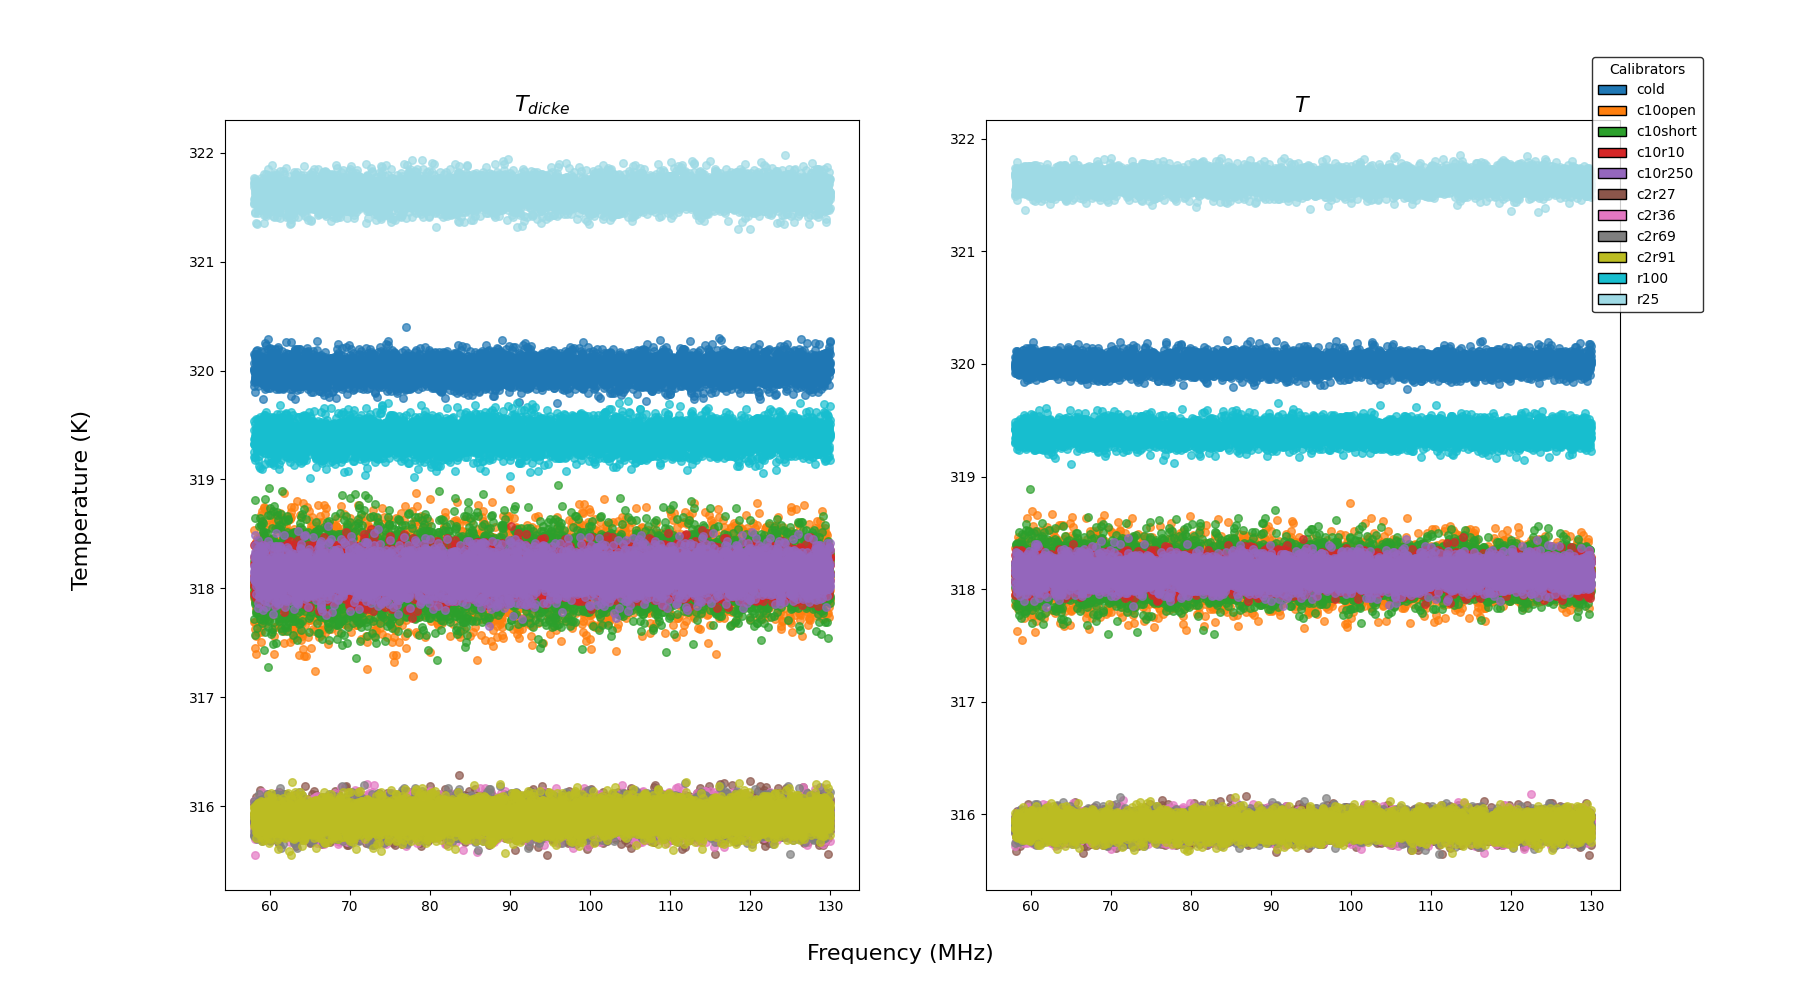
\includegraphics[width=1\textwidth]{main_scatter_plots.png}
				\label{fig:image1}
			\end{figure}
		\end{column}
	\end{columns}

\end{frame}


\begin{frame}
	\begin{figure}[h]
		\centering
		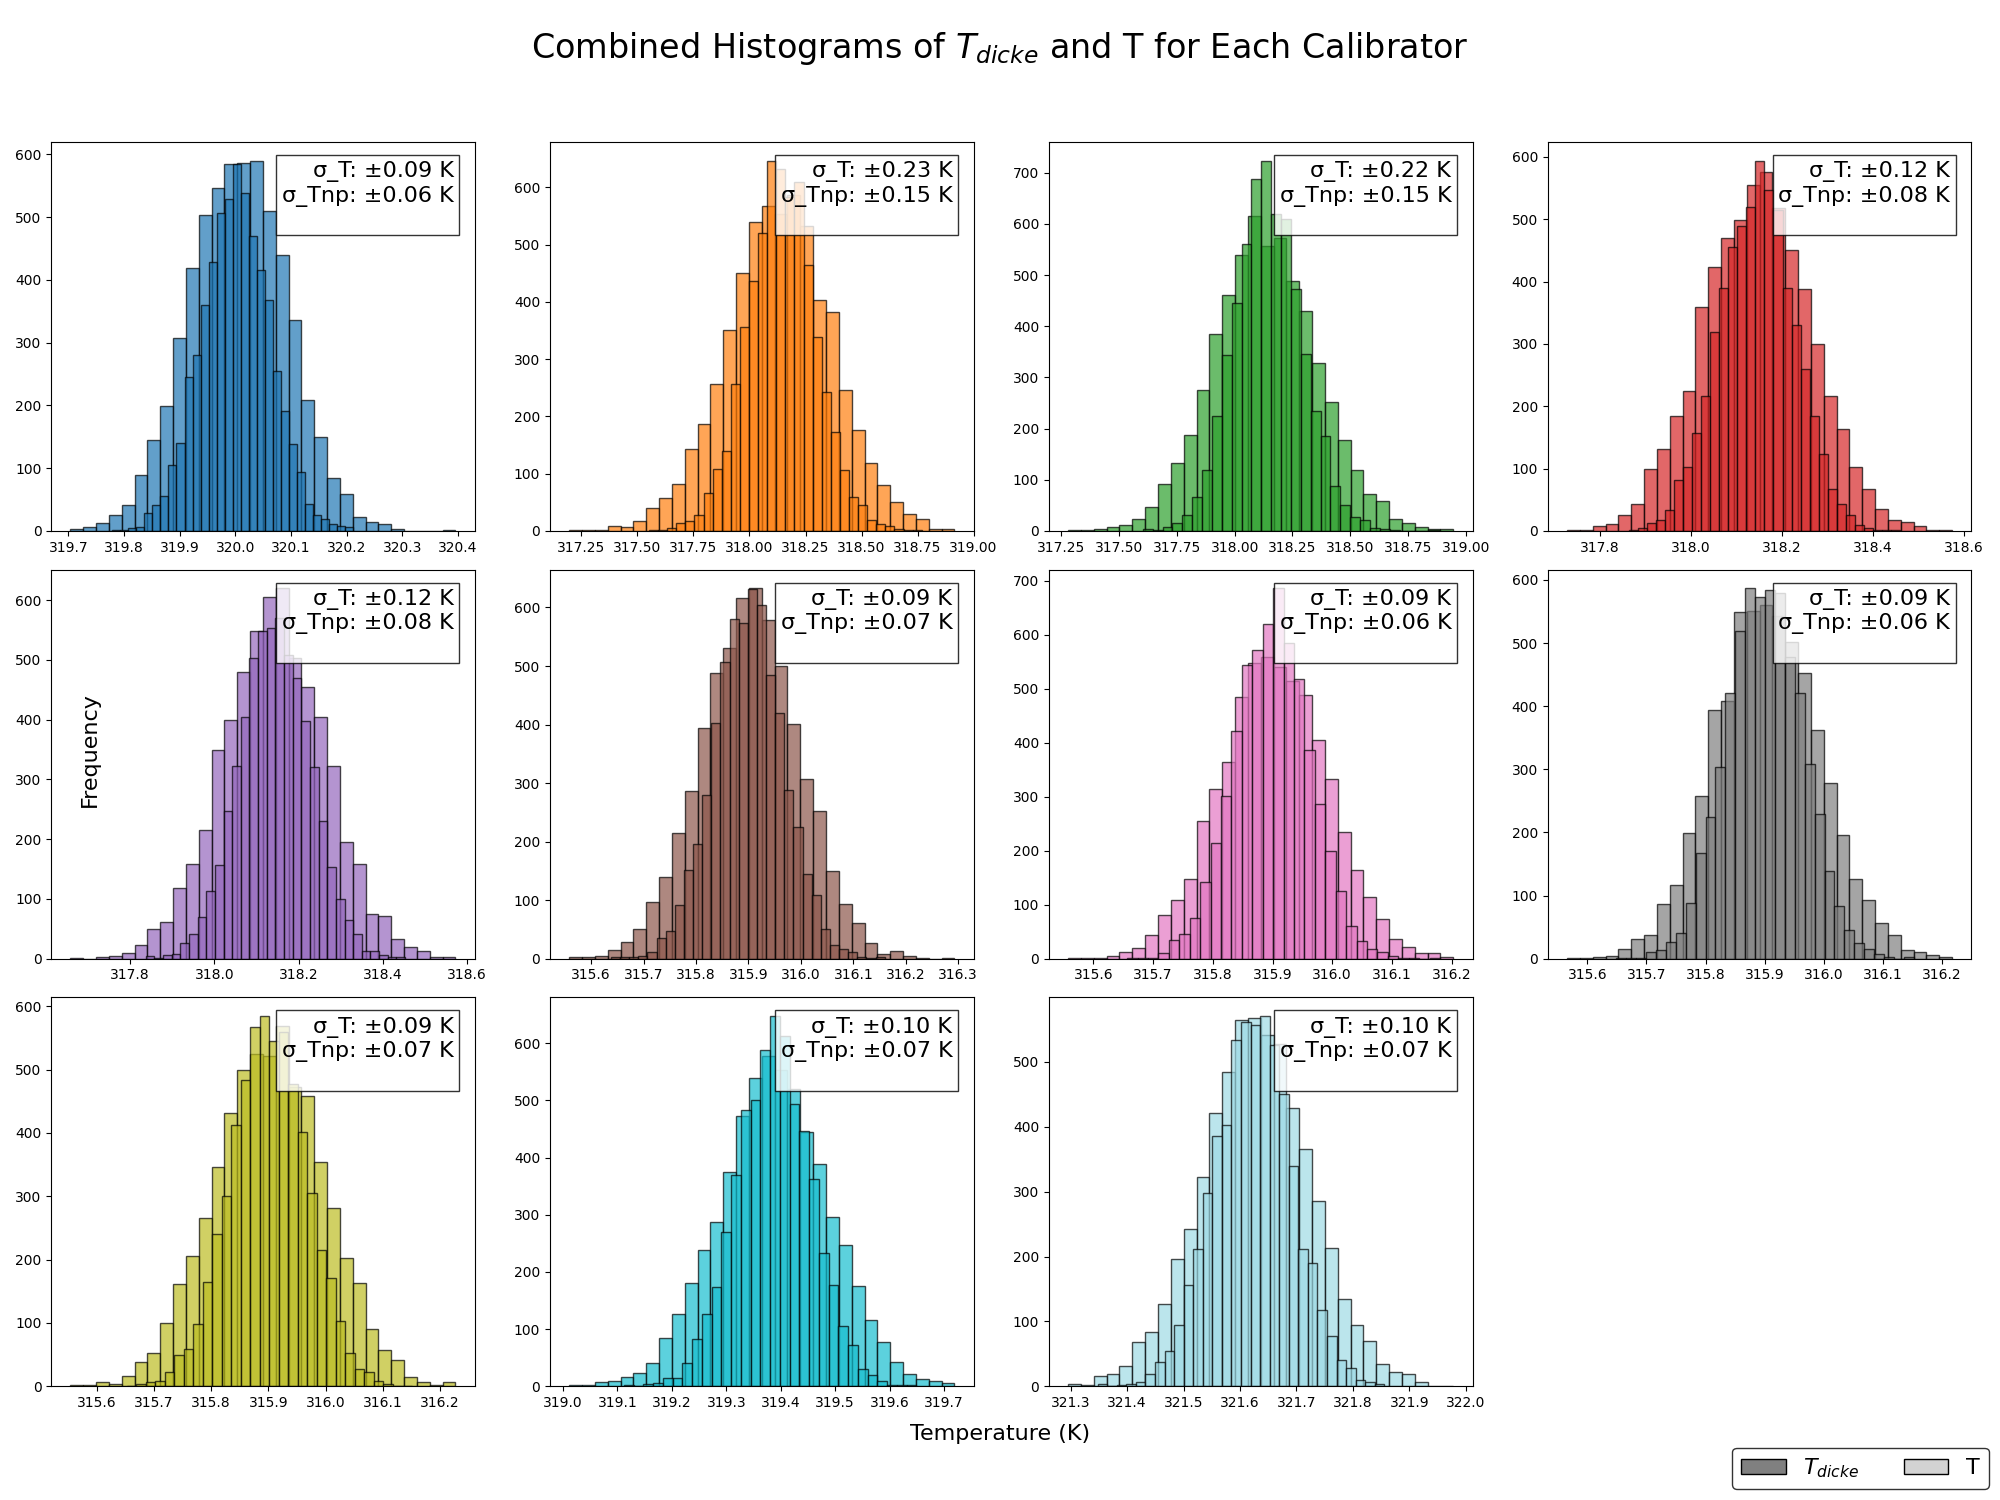
\includegraphics[width=0.8\textwidth]{combined_histograms.png}
		\label{fig:image2}
	\end{figure}
\end{frame}

\begin{frame}{Why not fit noise (wave) parameters directly?}

	% Noise Parameter Equation with smaller, uniform title
	\textbf{\small{Noise Parameter Equation:}}
	{\tiny
		\begin{equation}
			P_{\text{out}}^{\text{src}} = \textcolor{red}{g} M \left( T_{\text{in}}^{\text{src}} + \textcolor{red}{T_{\text{min}}} + T_0 \frac{4\textcolor{red}{R_N}}{Z_0} \frac{|\Gamma_{\text{src}} - \textcolor{red}{\Gamma_{\text{opt}}}|^2}{(1 - |\Gamma_{\text{src}}|^2)(1 + |\Gamma_{\text{opt}}|^2)} \right)
		\end{equation}
	}

	\vspace{0.3cm}
	\hrule  % Horizontal line for separation
	\vspace{0.3cm}

	% Noise Wave Equation with smaller, uniform title
	\textbf{\small{Noise Wave Equation:}}

	{\tiny
		\begin{multline}\label{}
			P_{\text{out}}^{\text{src}} = \textcolor{red}{g} \left[ \textcolor{red}{T_0} + \textcolor{red}{T_{\text{unc}}} |\Gamma_{\text{s}}|^2 \left|\frac{ \sqrt{1 - |\Gamma_{\text{rec}}|^2}}{1 - \Gamma_{\text{s}}\Gamma_{\text{rec}}} \right|^2 \right. \\
				\left. + T_{\text{s}}(1 - |\Gamma_{\text{s}}|^2) \left|\frac{ \sqrt{1 - |\Gamma_{\text{rec}}|^2}}{1 - \Gamma_{\text{s}}\Gamma_{\text{rec}}} \right|^2 + \textcolor{red}{T_{\text{cos}}} \Re \left( \Gamma_{\text{s}} \frac{\sqrt{1 - |\Gamma_{\text{rec}}|^2}}{1 - \Gamma_{\text{s}} \Gamma_{\text{rec}}} \right) \right. \\
				\left. + \textcolor{red}{T_{\text{sin}}} \Im \left( \Gamma_{\text{s}} \frac{\sqrt{1 - |\Gamma_{\text{rec}}|^2}}{1 - \Gamma_{\text{s}} \Gamma_{\text{rec}}} \right) \right]
		\end{multline}
	}

	\textit{We still end up with 5 unknowns, as before.}

\end{frame}


\begin{frame}{Machine learning}\footnotesize
	\begin{columns}
		\begin{column}{0.35\textwidth}
			\textbf{How/why?}
			\begin{itemize}
				\item Can predict noise wave parameters using machine learning.
				\item Could apply method to noise parameters.
				\item Predict \textbf{directly} on noise parameters on frequency by frequency basis.
				\item Maleable to environmental changes.
			\end{itemize}
		\end{column}
		\begin{column}{0.65\textwidth}
			\begin{figure}[h]
				\includesvg[width=0.9\textwidth]{mlcal.svg}
			\end{figure}
		\end{column}
	\end{columns}
\end{frame}

\begin{frame}{How to Calibrate with Machine Learning?}\footnotesize
	\begin{columns}
		% Left Column: Steps 1 and 2
		\begin{column}{0.5\textwidth}
			\textbf{1. Define the Loss Function}\\
			Regress over measured power and predicted power.\\
			\begin{equation}
				\mathcal{L} = \frac{1}{n}\sum_{i=1}^{n} \left( \mathcal{P}_{\text{measured},i} - \mathcal{P}_{\text{pred},i} \right)^{2}
			\end{equation}

			\vspace{0.5cm} % Adds vertical space between steps

			\textbf{2. Write Down the Equation for \(\mathcal{P}_{\text{pred}}\)}\\
			Using the noise wave formalism, relate \(\mathcal{P}_{\text{pred}}\) to \(T_{\text{src}}\).
			\begin{align}
				 & \mathcal{P}_{\text{pred}} = \textcolor{red}{g} \cdot M \left( T_{\text{in}}^{\text{src}} \right. \nonumber                                                                                                               \\
				 & \quad + \textcolor{red}{T_{\text{min}}} + T_0 \frac{4\textcolor{red}{R_N}}{Z_0} \frac{|\Gamma_{\text{src}} - \textcolor{red}{\Gamma_{\text{opt}}}|^2}{(1 - |\Gamma_{\text{src}}|^2)(1 + |\Gamma_{\text{opt}}|^2)} \Bigg)
			\end{align}
			\vfill
		\end{column}

		% Right Column: Step 3 with Definitions of Theta
		\begin{column}{0.5\textwidth}
			\textbf{3. Minimise the Loss Function}
			\begin{equation}
				\boldsymbol{\theta}^* = \arg\min_{\boldsymbol{\theta}} \mathcal{L}(\boldsymbol{\theta})
			\end{equation}
			parameter vector \(\boldsymbol{\theta}\) includes all tunable parameters in the model:
			\begin{equation}
				\boldsymbol{\theta} = \{ \textcolor{red}{g}, \textcolor{red}{T_{\text{min}}}, \textcolor{red}{R_N}, \textcolor{red}{\Gamma_{\text{opt}}^{\phi}}, \textcolor{red}{|\Gamma_{\text{opt}}|)}
			\end{equation}

			\textbf{4. Rearrange and Predict $(T_{\text{src}}$) using $\boldsymbol{\theta}^{*}$}
			\begin{align}
				T_{\text{src}} & = \frac{\mathcal{P}_{\text{pred}}}{\textcolor{red}{g^*} \cdot M} \nonumber \\
				               & \quad - \left( \textcolor{red}{T_{\text{min}}^*}
				+ T_0 \frac{4\textcolor{red}{R_N^*}}{Z_0} \frac{|\Gamma_{\text{src}} - \textcolor{red}{\Gamma_{\text{opt}}^*}|^2}{(1 - |\Gamma_{\text{src}}|^2)(1 + |\Gamma_{\text{opt}}^*|^2)} \right)
			\end{align}
			\vfill
		\end{column}
	\end{columns}
\end{frame}

\begin{frame}{The physical system}
	\begin{columns}
		\begin{column}{0.3\textwidth}
			\textbf{Process:}
			\begin{itemize}
				\item Switch between sources to generate training data.
				\item Calibration sources with known temperature train neural net.
				\item Predict $T_{\text{src}}$ of antenna.
			\end{itemize}
		\end{column}

		\begin{column}{0.7\textwidth}
			\begin{figure}
				\centering
				\includesvg[width=\textwidth]{instrument.svg}
			\end{figure}
		\end{column}
	\end{columns}
	\vfill
\end{frame}

\begin{frame}{Network Architecture}
	\begin{columns}
		\begin{column}{0.35\textwidth}
			\textbf{Structure:}
			\begin{itemize}
				\item Input thermistor and VNA measurments.
				\item Also input frequency.
				\item Predict noise parameters.
				\item Regress over loss function.
			\end{itemize}
		\end{column}

		\begin{column}{0.65\textwidth}
			\begin{figure}
				\centering
				\includesvg[width=\textwidth]{nn.svg}
			\end{figure}
		\end{column}
	\end{columns}
	\vfill
\end{frame}

\begin{frame}{Testing on simulated data with realistic antenna}
	\begin{figure}
		\centering
		\includesvg[width=1.05\textwidth]{results.svg}
	\end{figure}
\end{frame}


\begin{frame}{\small{General thoughts on REACH calibration}}
	\begin{itemize}
		\item We have tried 5 different 'data analysis' techniques.
		\item There are advantages and disadvantages but results are not drastically different.
		\item So what are we limited by?
		\item The conclusion of Ians thesis is that we are limited by the quality of specific Physical measurments of the system (namely cable measurments and switches).
		\item I do not think Dicke switching is needed at all - can someone convince me otherwise?
	\end{itemize}

\end{frame}

\begin{frame}{\small{Thank you!}}
	\begin{figure}
		\centering
		
\includegraphics[width=0.45\textwidth]{qr.png}
	\end{figure}
\end{frame}

\end{document}
